\documentclass[runningheads]{llncs}
\usepackage{graphicx}
\graphicspath{ {./images/} }
\usepackage[export]{adjustbox}
\usepackage{tcolorbox}



\title{
    Retele de calculatoare\\
    Raportul tehnic al proiectului\\
    Smart Parking Assistant
    }
\author{Ciotir Marian-Augustin}
\date{11 Decembrie 2023}
\institute{Facultatea de Informatica Iasi}
\textwidth=14cm
\renewcommand{\refname}{}
\begin{document}
\maketitle

\section{Introducere}
\subsection{Viziunea generala a proiectului}
Cu totii stim cat de aglomerate pot fi parcarile mai ales in perioada sarbatorilor si cat de greu este sa gasim un loc de parcare liber si sa avem ocazia sa il ocupam. De aceea am ales acest proiect pentru a face acest proces mai usor prin crearea unei aplicatii care permite soferilor sa isi gaseasca un loc de parcare liber cu usurinta.
\subsection{Obiectivele proiectului}
Acest proiect are obiectivul de a ajuta soferii sa gaseasca un loc de parcare liber in special in parcarile aglomerate prin intermediul unei interfete care le permite sa vizioneze locurile libere din parcare si sa isi rezerve unul din acestea, fara a mai fi nevoie sa faca turul unei parcari in cautarea unui loc liber.

\section{Tehnlogii utilizate}
Aplicatia ``Smart Parking Assistant'' este realizata in limbajul de programare C++, comunicarea dintre client si server fiind realizata prin socket-uri, iar ca protocol de comunicare am ales TCP deoarece este un protocol orientat pe conexiune si asigura o comunicare sigura intre client si server. De asemenea, acest protocol ofera o conexiune de calitate intre client si server, permite transmiterea de date in ambele sensuri, detectarea erorilor de transmsie, retransmiterea pachetelor pierdute, si nu in ultimul rand, permite transmiterea datelor in ordinea in care au fost trimise. Aceste aspecte sunt necesare pentru proiectul ales deoarece este nevoie de o actualizare in timp real cat mai precisa si rapida a situatii locurilor de parcare. Pentru tratarea concurenta a clientilor am folosit thread-uri, iar ca interfata grafica am folosit biblioteca grafica SFML.\\
\pagebreak
\section{Structura aplicatiei}

Aplicatia este alcatuita din 3 componente: client, server, si camera care va fi simulata cu ajutorul unui client special care va actualiza situatia unor locuri de parcare la un timp aleator T. In cadrul aplicatiei, clientul va putea vizualiza situatia in timp real a locurilor de parcare, alaturi de numarul exact acestora. Clientul va putea rezerva un loc de parcare, iar in cazul plecarii acestuia, il va putea elibera.

Figura 1 reprezinta o figura a interfetei aplicatiei.
\begin{center}
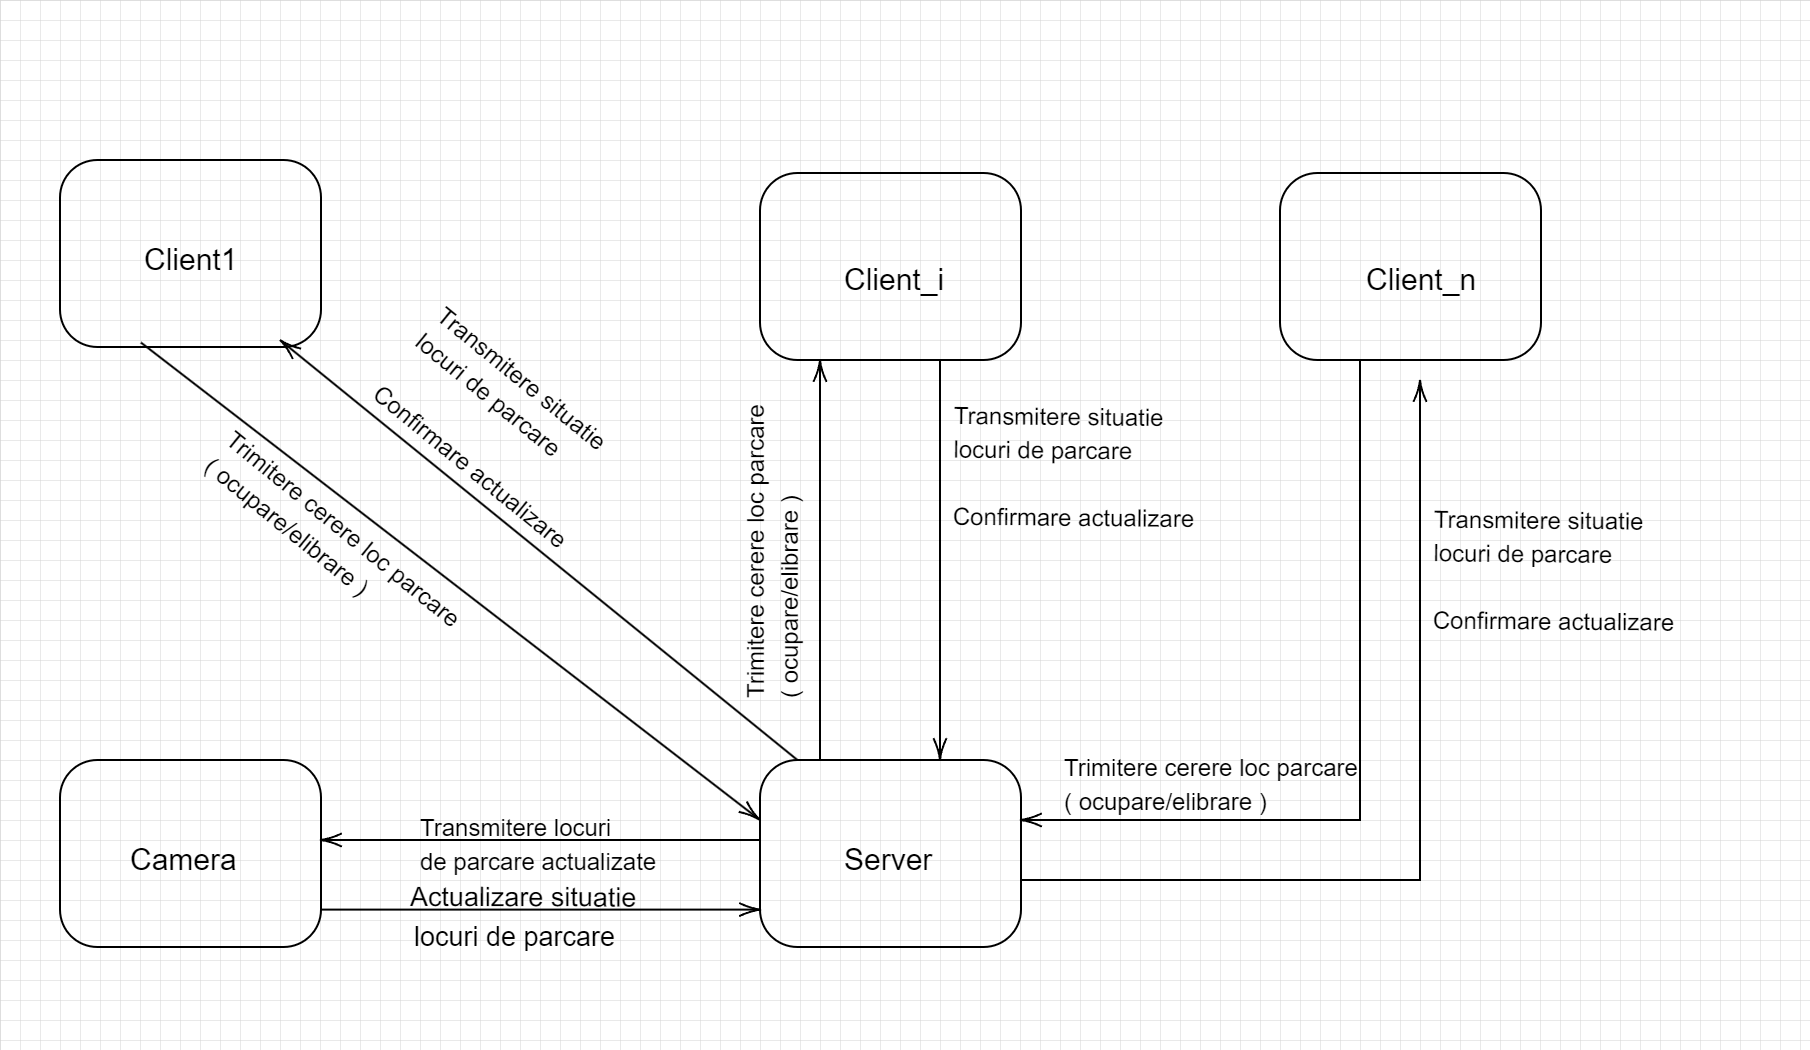
\includegraphics[width=\linewidth, height=11cm]{fig1.png}
\end{center}

\section{Aspecte de implementare}

O seciune de cod specifica proiectului este cea de mai jos, unde avem un exemplu de parcare cu 144 de locuri, impartite pe 6 sectiune de cate 24 de locuri. Am folosit tip de date bool pentru a tine cont de starea locului (liber=0, ocupat=1). Mai jos este sectiunea de procesare a cererii de ocupare sau elibrare a unui loc de parcare.
\begin{tcolorbox}[colback=red!5,colframe=red!50!black,width = \linewidth, title = Cerere ocupare/eliberare loc de parcare]
    \begin{verbatim}

    if (strstr(message, "vreau") != NULL)
    {
        {
            std::cout<<"Am primit cerere de parcare\n";
            int i, j;
            guard.lock();
            do
            {
                i = rand() % 6;
                j = rand() % 24;
            } while (parcare[i][j] == 1);
            parcare[i][j] = 1;
            guard.unlock();
            flag.notify_all();
            sprintf(response, "vreau %d %d\n", i, j);
            if (write(camera, response, strlen(response)) <= 0)
            {
                perror("[server]Eroare la write() catre camera.\n");
                continue;
            }
            strcpy(response, "Ai primit locul de parcare: ");
            strcat(response, loc_parcare(i, j).c_str());
            data->parkingSlot.i = i;
            data->parkingSlot.j = j;
        }
    }
    
    else if (strstr(message, "eliberez") != NULL)
    {
        std::cout<<"Eliberez locul de parcare\n";
        guard.lock();
        parcare[data->parkingSlot.i][data->parkingSlot.j] = 0;
        sprintf(response, "eliberez %d %d\n", data->parkingSlot.i,
        data->parkingSlot.j);
        if (write(camera, response, strlen(response)) <= 0)
        {
            perror("[server]Eroare la write() catre camera.\n");
            continue;
        }
        data->parkingSlot.i = -1;
        data->parkingSlot.j = -1;
        guard.unlock();
        flag.notify_all();
        strcpy(response, "Ai eliberat locul de parcare cu succes!");
    }
    std::cout<<"[server]Mesajul a fost trasmis cu succes.\n";
\end{verbatim}
\end{tcolorbox} 

O alta sectiune de cod importanta pentru proiect este trimiterea situatiei locurilor de parcare de la camera la server. Locurile sunt trimise sub forma unui string de 144 de caractere, unde 0 reprezinta un loc liber, iar 1 reprezinta un loc ocupat. De asemenea de fiecare data cand se face o actualizare, situatia locurilor este salvata intr-un fisier $.txt$ la care camera are acces in caz de restart.
\begin{tcolorbox}[colback=red!5,colframe=red!50!black,width = \linewidth, title = Transmitere situatie locuri de parcare]
\begin{verbatim}
    int length = 0;
    message[0] = '\0';
    std::ofstream fout("parking_state.txt", std::ios::out |
    std::ios::trunc);
    for (int i = 0; i < 6; ++i)
    {
        for (int j = 0; j < 24; ++j)
        {
            message[length++] = parcare[i][j] ? '1' : '0';
            fout << (parcare[i][j] ? '1' : '0');
        }
    }
    fout.close();
    message[length] = '\0';
    if (write(socket_desc, message, length) < 0)
    {
        perror("[camera]Eroare la send().\n");
        return errno;
    }\end{verbatim}
\end{tcolorbox}
\section{Concluzii}

Un element ce poate imbunatati calitativ folosirea aplicatiei este o interfata grafica imbunataita care ar fi mai placuta si atractiva pentru utilizator. O alta imbunatatire ce poate fi adusa aplicatiei ar putea fi folosirea unei baze de date 

\section{Bibliografie}
\begin{thebibliography}{}
    \bibitem{}
    https://profs.info.uaic.ro/~gcalancea/lab7/servTcpConc.c
    \bibitem{}
    https://www.mathcha.io/editor
    \bibitem{}
    https://www.sfml-dev.org/documentation/2.6.1/
    \bibitem{}
    https://en.cppreference.com/w/
    \end{thebibliography}

\end{document}